\documentclass[a4paper,10pt]{article}

%set font to Arial
%\usepackage{fontspec}
%\setmainfont{Arial}
\usepackage{helvet}
\renewcommand{\familydefault}{\sfdefault}

%graphics
\usepackage{graphicx}
%\usepackage{subfigure}
\usepackage{pslatex}
\usepackage{pstricks}

%math equations
\usepackage{amsmath}

%python code
%\usepackage{minted}

%glossary
\usepackage[toc]{glossaries}
\makeglossary

%appendix
\usepackage[title,titletoc,toc]{appendix}

%headers
\usepackage{lastpage}
\usepackage{fancyhdr}
\pagestyle{fancy} 
\lhead{IRAS Project ID: 203355}
\chead{}
\rhead{clinicaltrials.gov: NCT03211507}
\lfoot{IPFJES}
\cfoot{Study Protocol v0.6 \hspace{2cm} 29th September, 2017}
\rfoot{\thepage\ of \pageref{LastPage}} 


%display URLS
\usepackage{url}

%hyperlinks
\usepackage{hyperref}

%comments
\usepackage{verbatim} 

%nice tables
\usepackage{booktabs}
\newcommand{\ra}[1]{\renewcommand{\arraystretch}{#1}}

%multi rows for the nice tables
%\usepackage{multirow} 

%nice diplay of code
%\usepackage{minted}

%nice references
\usepackage[super]{natbib}

%some maths
\usepackage{amsmath}

%ability to include pdf
\usepackage{pdfpages}

%captions
\usepackage{caption}

%margins
%\usepackage{geometry}
%\geometry{verbose,a4paper,tmargin=60mm,bmargin=25mm,lmargin=25mm,rmargin=25mm}

%in line citations
%\usepackage{bibentry}

%\hyphenpenalty=10000

%\nobibliography*


\newpage
\title{\bf IPF JES} 
\date{}

%\pagenumbering{gobble}

%don't have to change study dates everywhere
\newcommand{\studystart}{February 2017 }
\newcommand{\studyend}{October 2019 }

\begin{document}
\pagestyle{fancy} 

%\pagestyle{empty}

\maketitle



\section*{Idiopathic Pulmonary Fibrosis Job Exposures Study}
 \subsection*{A case-control study to investigate whether occupational asbestos exposure is an under-recognized cause of idiopathic pulmonary fibrosis (IPF) using an interview to measure previous
asbestos exposure and a blood test to investigate genetic susceptibility.}


\begin{centering}
\subsection*{Version 0.6 \\ 29th September, 2017}
\end{centering}

\begin{flushleft}

\vspace{3cm}

MAIN SPONSOR: Imperial College London \\
FUNDERS: Wellcome Trust (201291/Z/16/Z) \\
STUDY COORDINATION CENTRE:  Imperial College London \\
IRAS reference: 203355\\

\vspace{3cm}

\subsection*{Protocol authorised by:}

    \begin{tabular}{l c r}
        Name \& Role & Date & Signature \\
        Carl Reynolds, Chief Investigator & 29th September, 2017 & \includegraphics[scale=0.6]{/home/drcjar/Documents/CV/CarlReynoldsSignature.png} \\

    \end{tabular}



\newpage

\subsection*{Study management group}

Chief Investigator: Carl Reynolds

Co-investigators: Paul Cullinan, Chris Barber, Sara De Matteis

Statistical Supervisor: Cosetta Minelli

Statistician: Carl Reynolds

Study Management: Paul Cullinan, Chris Barber, Sara De Matteis, Carl Reynolds

\subsection*{Study Coordination Centre}

For general queries, supply of study documentation, and collection of data, please contact: \vspace{0.6cm}

Dr Carl Reynolds 

carl.reynolds@imperial.ac.uk 

07737 904 807 

National Heart and Lung Institute

Room G39 Emmanual Kaye Building

1b Mansrea Road, London, SW3 6LR 


\subsection*{Clinical Queries}

Clinical queries should be directed to Dr Carl Reynolds who will direct the query to the appropriate person.

\subsection*{Sponsor}

Imperial College London is the main research Sponsor for this study. For further information regarding the sponsorship conditions, please contact the Head of Regulatory Compliance at:\vspace{0.6cm}
		
Joint Research Compliance Office

Imperial College London \& Imperial College Healthcare NHS Trust

2nd Floor Medical School Building

St Mary’s Hospital
Praed Street
London
W2 1NY

Tel: 020159 41862

\subsection*{Funder}


Wellcome Trust (Ref 201291/Z/16/Z) \vspace{0.6cm}

\end{flushleft}


This protocol describes the Idiopathic Pulmonary Fibrosis Job Exposures Study (IPF JES) and provides information about procedures for entering participants. Every care was taken in its drafting, but corrections or amendments may be necessary. These will be circulated to investigators in the study. Problems relating to this study should be referred, in the first instance, to the Chief Investigator. This study will adhere to the principles outlined in the NHS Research Governance Framework for Health and Social Care (2nd edition). It will be conducted in compliance with the protocol, the Data Protection Act and other regulatory requirements as appropriate. 

\newpage
 
\tableofcontents

\newpage

\newglossaryentry{Idiopathic pulmonary fibrosis}
  {name=Idiopathic pulmonary fibrosis,
  description={Idiopathic pulmonary fibrosis (IPF) is a disease that causes scarring of the lungs. The `idiopathic' part of the name refers to the cause of the disease being unknown}}


\newglossaryentry{Asbestos}
{name=Asbestos,
 description={Asbestos is a mineral fibre with useful insulating properties. Asbestos use is now strictly controlled because of harmful health effects. Historically, construction materials and household goods have been made from asbestos, and widely used, in the United Kingdom}}

\newglossaryentry{Case-control study}
{name=Case-control study,
 description={A Case-control study is an observational epidemiological study of persons with a disease of interest and a suitable control group of persons without the disease. The relationship of a suspected risk factor to disease is examined by comparing exposure to the risk factor in the two groups}}

%need to do something to actually build the glossary...%

\glsaddall

\printglossary[nonumberlist]

\section*{Key words}

\textbf{Idiopathic pulmonary fibrosis, asbestos, case-control study}

\newpage

\section*{Study Summary}
\addcontentsline{toc}{section}{Study Summary}

\paragraph{Title:} Idiopathic Pulmonary Fibrosis Job Exposures Study (IPF JES).
\paragraph{Design:} Hospital case-control study.
\paragraph{Aim:} To characterize and measure asbestos exposure as an occupational determinant of IPF.
\paragraph{Outcome measures:} 1. Association between asbestos exposure and IPF estimated using logistic regression for ‘any’ vs ‘no’ asbestos exposure and categories of cumulative exposure and adjusting for age and smoking status. 2. Gene-environment interaction (for MUC5B rs35705950 and asbestos exposure) odds ratio.
\paragraph{Population:} Male patients with a new diagnosis of IPF and age-matched controls who have a new outpatient clinic appointment during the study period.
\paragraph{Eligibility:} Meets population definition, able to give informed consent, has never worked outside of the UK.
\paragraph{Duration:} Three years.


\newpage


\section{Introduction}
\subsection{Background}

Idiopathic pulmonary fibrosis (IPF) is a progressive, fibrotic lung disease which in 2012 was the recorded cause of death for c.4000 people in England/Wales. Its incidence, currently around 7.5/100,000 person-years, has increased by 5\% pa since 2000.\cite{Navaratnam2011} The pathophysiology of IPF is complex, the outcome of host susceptibility factors, epithelial injury, and a dysregulated repair process. Several gene polymorphisms which result in a vulnerable alveolar epithelium have been characterized; they include abnormalities in mucin genes (eg MUC5B), surfactant protein genes, and telomerase genes (eg TERT and TERC).\cite{Maher2012}\cite{Ley2013}\cite{Spagnolo2004} The median age of onset is 70 years and the condition is more common in men (M:F ratio 1.6), manual workers, and those living in industrial areas\cite{Navaratnam2011}, patterns that are not unique to the UK.\cite{Ley2013} The prognosis is poor, with a median survival of three years.\cite{Hubbard1998}\cite{Vancheri2010} 

These epidemiological distributions of IPF are consistent with a long-latency response to occupational dust exposure; in particular, the incidence of IPF correlates strongly (if ecologically) with historic asbestos use.\cite{Barber2015} Mineralogical studies support the concept of asbestosis-IPF misclassification by revealing high fibre burdens in the lung tissue of patients diagnosed with `IPF' and revision of the diagnosis to `asbestosis'.\cite{Monso1990}\cite{Monso1991}\cite{Glazer2009}\cite{Ghio2004} 

Identification of occupational asbestos fibre exposure as an under-recognized cause of IPF is important to improve our understanding of the aetio-pathophysiology of IPF and the accuracy of prognostic information. It would have implications for compensation and impact on the current restrictions on individual treatment. Importantly, it would inform evidence-based workplace exposure policies in the UK and internationally, particularly in the many countries with continuing high levels of asbestos use. Details of how the proposed research will inform government policy and change working practices are provided in Appendix A.

In preparing this protocol, I examined mortality trends in England and Wales for IPF and asbestos-related diseases. UK age-standardized mortality rates from 1974 to 2012 continued to rise with marked sex and regional variations, consistent with occupational exposure being an under-recognized cause of IPF.\cite{Reynolds2015} I analysed European age-standardised mortality rates for mesothelioma and IPF for 27 countries for which data was available and found a positive correlation (r = 0.61, p = 0.007). I collated 13 case-control studies of IPF and occupational dust exposure; eight reported significant associations with metal dust exposure \cite{Scott1990}\cite{Iwai1994}\cite{Hubbard1996}\cite{Hubbard2000}\cite{Miyake2015}\cite{Pinheiro2008}, four with wood dust \cite{Hubbard1996a}\cite{Gustafson2007}\cite{Pinheiro2008}\cite{Awadalla2012} and two with stone dust.\cite{Baumgartner2000}\cite{Mullen1998}

Finally, I analysed the limited occupational information in a recent case-control study, designed to examine the role of thrombosis in IPF.\cite{Navaratnam2011} Using an approach from a large mesothelioma study based on proportional mortality ratios\cite{Rake2009} I estimated the odds ratio (OR) associated with ever having had a job with probable asbestos exposure was 2.8 (95\% CI: 1.42-5.75, p = 0.001) adding further weight to the argument that occupational asbestos exposure in IPF should be properly investigated. Supplementary figures and a table of previous case-control studies are provided in Appendix B. 

In addition to its epidemiological and clinical plausibility there are several additional reasons why study of this area is needed. First, most previous work relied on self-reported workplace exposure information, an approach that is open to recall bias and deals poorly with confounding; for example, studies have described strong associations between metal work and IPF and specify sheet metal workers\cite{Iwai1994}\cite{Scott1990}\cite{Hubbard2000}, a group who are frequently exposed to dust
containing asbestos fibres\cite{Welch1994} and who in a recent UK study, had the highest risk of mesothelioma.\cite{Rake2009} Lifetime occupational histories are more accurately recalled than self-reported workplace exposures and can be combined with measures such as proportionate mortality (PMR) estimates and job-process assessments to minimize recall bias and more accurately characterise cumulative exposures.
\cite{Teschke2002}\cite{Bourgkard2013}\cite{Cherrie1999}\cite{Rake2009}\cite{Gilham2015} This allows too the examination of `exposure-response' relationships, entirely lacking in the published literature. 

Second, all but two studies\cite{Iwai1994}\cite{Awadalla2012} used community controls. While this is generally desirable, ‘hospital’ controls are preferred in circumstances when acceptable community control participation rates cannot be achieved, case acquisition is incomplete, or recall bias is an issue. Recent participation rates for community controls in UK studies of IPF have been as low as 28\%;\cite{Navaratnam2015} and a recent US series estimated that the ante-mortem diagnosis of IPF was missed in 20\% of cases.\cite{Daniels2008} Further, the use of community controls for hospital cases risks significant information mismatch on exposures. While hospital controls are less representative of the base population, their use does not prevent a study from being either scientifically valid or generalizable\cite{Rothman2013} as is well demonstrated by a recent influential UK hospital case-control study which found that exposure to metal fume predisposed to infectious pneumonia.\cite{Palmer2003}

Third, advances in our understanding of IPF susceptibility now permit study of host-exposure interactions. The minor-allele of the rs35705950 SNP in the mucin 5B gene was found to be present in 38\% of IPF patients but just 9\% of controls.\cite{Seibold2011} The polymorphism results in excess MUC5B protein in the airway, impaired clearance of inhaled substances and a chronic inflammatory burden on the alveolar surface.\cite{Seibold2011}  The association is allele dose-dependent, has been replicated in independent cohorts, and appears to confer improved survival.\cite{Ley2013}\cite{Seibold2011}\cite{Peljto2013} Two large GWASs have confirmed the observed associations of IPF with MUC5B and other loci.\cite{Fingerlin2013}\cite{Noth2013}

I propose a new case-control study that systematically collects lifetime occupational histories to derive exposure risk using formal asbestos exposure assessment. I will also collect IPF susceptibility genotypes to permit me, uniquely, to examine exposure-response relationships, latency periods and genotype-exposure interactions. 

\section{Study objectives}
My overall aim is to characterize and measure asbestos exposure as an occupational determinant of IPF; additionally, I will determine host-exposure interactions mediated by candidate susceptibility polymorphisms (in particular MUC5B promoter polymorphism rs35705950). 

My specific research questions are:
\begin{enumerate}
 \item Does a dose-response relationship exist for occupational asbestos exposure and IPF? 
 \item Does the presence of asbestos exposure modify the association between IPF and rs35705950? 
\end{enumerate}

\section{Study design}
\subsection{Study outcome measures}
\paragraph{Primary outcome}
Association between asbestos exposure and IPF estimated using logistic regression for ‘any’ vs ‘no’ asbestos exposure and categories of cumulative exposure and adjusting for age and smoking status.

\paragraph{Secondary outcome}
Gene-environment interaction odds ratio (for MUC5B rs35705950 and asbestos exposure)

\section{Participant entry}
\subsection{Pre-registration evaluations}
Pre-registration evaluation will include screening for eligibility using inclusion and exclusion criteria.

\subsection{Sampling}
Cases and controls will be frequency matched on age categories.

\subsection{Inclusion criteria}
\begin{itemize}
 \item Cases \begin{itemize}
        \item Male
        \item New diagnosis of IPF between \studystart and \studyend 
       \end{itemize}
       
  \item Controls \begin{itemize}
        \item Male
        \item Outpatient department attendee between \studystart and \studyend
       \end{itemize}

\end{itemize}


\subsection{Exclusion criteria}
\begin{itemize}
 \item Cases \begin{itemize}
        \item Unable to give informed consent
        \item Worked outside of the UK for one year or more (does not include work outside the UK by member of the armed forces or merchant navy)
       \end{itemize}
       
  \item Controls \begin{itemize}
        \item Unable to give informed consent
        \item Worked outside of the UK for one year or more (does not include work outside the UK by member of the armed forces or merchant navy)
       \end{itemize}

\end{itemize}


\subsection{Withdrawal criteria} 
Research participants will be withdrawn from the study upon their request or if for any reason they are unable to complete the study interview. 

\section{Adverse events}

\subsection{Definitions}

\paragraph{Adverse Event (AE):}any untoward medical occurrence in a patient or clinical study subject.  

\paragraph{Serious Adverse Event (SAE):}any untoward and unexpected medical occurrence or effect that: \begin{itemize}
	\item Is life-threatening – refers to an event in which the subject was at risk of death at the time of the event; it does not refer to an event which hypothetically might have caused death if it were more severe
	\item Requires hospitalisation, or prolongation of existing inpatients’ hospitalisation
    \item Results in persistent or significant disability or incapacity
	\item Is a congenital anomaly or birth defect
                                                                                              \end{itemize}


Medical judgement should be exercised in deciding whether an AE is serious in other situations. Important AEs that are not immediately life-threatening or do not result in death or hospitalisation but may jeopardise the subject or may require intervention to prevent one of the other outcomes listed in the definition above, should also be considered serious.

\subsection{Reporting Procedures}
All adverse events should be reported. Depending on the nature of the event the reporting procedures below should be followed. Any questions concerning adverse event reporting should be directed to the Chief Investigator in the first instance.  

\subsubsection{Non serious AEs}
An SAE form should be completed and emailed to the Chief Investigator within 24 hours. However, relapse and death due to IPF, and hospitalisations for elective treatment of a pre-existing condition do not need reporting as SAEs.

All SAEs should be reported to the Imperial College London where in the opinion of the Chief Investigator, the event was: \begin{itemize}
                                                                                                                           \item ‘related’, ie resulted from the administration of any of the research procedures; and
					   \item ‘unexpected’, ie an event that is not listed in the protocol as an expected occurrence
                                                                                                                         \end{itemize}

                                                                                                                          
Reports of related and unexpected SAEs should be submitted within 15 days of the Chief Investigator becoming aware of the event, using the NRES SAE form for non-IMP studies. The Chief Investigator must also notify the Sponsor of all SAEs.

Local investigators should report any SAEs as required by their Local Research Ethics Committee, Sponsor and/or Research \& Development Office.

\begin{center}
\textbf{Contact details for reporting SAEs:}
 
Email: carl.reynolds@imperial.ac.uk

Please send SAE forms to: 

National Heart and Lung Institute

Room G39 Emmanual Kaye Building

1b Mansrea Road, London, SW3 6LR 

Tel: 07737 904 807

\end{center}


\section{Assessment and follow up}
Research participants will complete an interview and a blood test. The study will end when analysis of the last research participant is complete.

\section{Statistics and data analysis}
For the primary analysis logistic regression will be used to analyse ‘any’ vs ‘no’ asbestos exposure and
categories of cumulative exposure adjusting for age and smoking status. Prior data indicate that the probability of
exposure among controls is 0.63. If the true OR for disease in exposed subjects relative to unexposed subjects is 1.5,
I will need to recruit 460 case patients and 460 control patients to be able to reject the null hypothesis that this odds
ratio equals 1 with \ensuremath{\beta = 0.2} and \ensuremath{\alpha = 0.05}; my planned sample size includes a margin for model stability
and incomplete data.

Secondary (exploratory) analysis will investigate gene-environment interaction. The global minor allele frequency of
MUC5B rs35705950 is 0.05. With an estimated prevalence of IPF of 20/100000 and with ORs 1.5 for asbestos exposure 
and 6.8 for rs35705950, 460 cases would be required to detect a minimum interaction OR of 5.0.

\section{Regulatory issues}

\subsection{Ethics approval}
The Chief Investigator has obtained approval from the Research Ethics Committee via IRAS\@. The study must be submitted for Site Specific Assessment (SSA) at each participating NHS Trust. The Chief Investigator will require a copy of the Trust R\&D approval letter before accepting participants into the study. The study will be conducted in accordance with the recommendations for physicians involved in research on human subjects adopted by the 18th World Medical Assembly, Helsinki 1964 and later revisions.


\subsection{Consent}
Consent to enter the study will be sought from each participant only after a full explanation has been given, an information leaflet offered, and time allowed for consideration. Signed participant consent will be obtained. The right of the participant to refuse to participate without giving reasons will be respected. In these cases the participant will be withdrawn from the study and their data and samples destroyed. All participants are free to withdraw at any time from the protocol treatment without giving reasons and without prejudicing further treatment.

\subsection{Confidentiality}
The Chief Investigator will preserve the confidentiality of participants taking part in the study and is registered under the Data Protection Act.

\subsection{Indemnity}
Imperial College London holds negligent harm and non-negligent harm insurance policies which apply to this study.

\subsection{Sponsor}
Imperial College London will act as the main Sponsor for this study. Delegated responsibilities will be assigned to the NHS trusts taking part in this study.  


\subsection{Funding}
The Wellcome Trust are funding the research.

\subsection{Audits and inspections}
The study may be subject to inspection and audit by Imperial College London under their remit as sponsor and other regulatory bodies to ensure adherence to GCP and the NHS Research Governance Framework for Health and Social Care (2nd edition). 

\section{Study management}
The day-to-day management of the study will be co-ordinated through Dr Carl Reynolds.

\section{Publication policy}
All research findings will be published in accordance with the Wellcome Trust and Imperial College London open access publication policies.

\newpage

\begin{appendices}

\section{Research outputs}

There will be three main outputs of the study:

\begin{enumerate}
 \item Data from the study, including anonymised raw data, will be communicated to the wider academic community,
and policy-makers, by publication and presentation at national and international respiratory and epidemiology
meetings.
 \item Data from the study will inform HSE and policy decisions with respect to work place dust control; we are
collaborating with Andrew Darnton who works at HSE specialising in mesothelioma and other asbestos related
diseases.
 \item Data from the study will inform policy decisions with respect to the use of anti-fibrotic treatments in patients
with asbestosis. We will establish good working relations with NICE
and the NHS England Specialist Respiratory Clinical Reference Group to communicate our findings.
NHS patients with IPF due to occult occupational asbestos exposure may be entitled to compensation and our
work may lead to reconsideration of current restrictions on disease modifying anti-fibrotic therapies for patients
with asbestosis.
\end{enumerate}

An estimated 125 million people around the world work in environments in which they are exposed to asbestos,
and at least 107,000 people die from occupational exposure to asbestos every year\cite{Concha-Barrientos2015}. Understanding the role of
asbestos exposure in idiopathic pulmonary fibrosis is an important data point for disease prevention policy
measures.

\newpage

\section{Supplementary figures and tables}

\begin{figure}[htp]
\centering
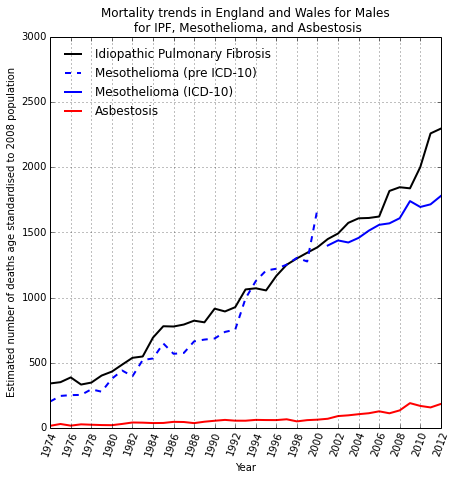
\includegraphics[width=12cm,height=10cm]{fig/uk-ipf-meso-asb-mortality-trends.png}
\caption{ONS data. Idiopathic Pulmonary Fibrosis, Mesothelioma, and Asbestosis mortality trends for England and Wales 1974-2012. A corrective factor provided by HSE has been applied to pre-ICD 10 Mesothelioma deaths (dashed line). https://github.com/drcjar/pypf/blob/master/notebooks/pypf\_analysis.ipynb}
\end{figure}

\newpage

\begin{figure}[htp]
\centering
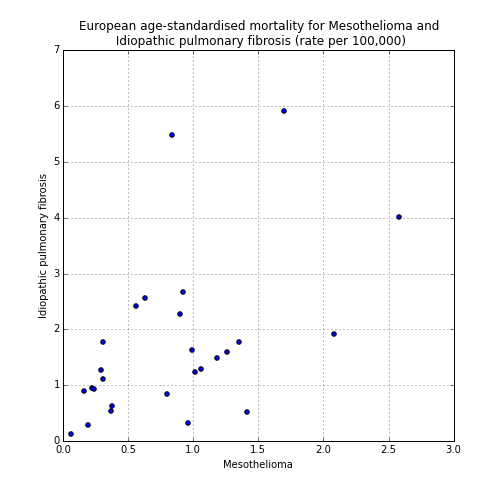
\includegraphics[width=12cm,height=10cm]{fig/european-meso-ipf-assoc.png}
\caption{ERS Whitebook data. Age standardised mortality rate per 100,000 for 27 European Union member countries (data not available for Greece). Pearson correlation coefficient = 0.61, p = 0.007. https://github.com/drcjar/pypf/blob/master/notebooks/ERS\_whitebook\_ipf\_meso.ipynb}
\end{figure}

\newpage

\begin{table}[htbp]\centering
\caption*{Summary of case-control studies of occupational dust exposure in IPF by Carl Reynolds}


\label{OccupationalDustTable1}
\tiny	
\begin{tabular}{p{1.3cm}p{0.8cm}p{0.8cm}p{6cm}p{5cm}}
\toprule
\textbf{Ref} & \textbf{Country} & \textbf{Cases (N)} & \textbf{Findings} & \textbf{Notes (including source of cases and controls, measure of exposure used, and response rates)}\\
\midrule

Scott 1990 & UK & 40 & Occupational exposures to metal dust ((OR 10.97, 95\%CI 2.3-52.4, p\ensuremath{<}0.001), wood dust (OR 2.94, 95\%CI 0.87-9.9), p = 0.08), and stone/sand (OR 1.59, 95\%CI 0.62-4.79) are associated with IPF & Community controls, questionnaire asking directly about exposures, response rate was 87\% for cases and 60\% for controls.\\


Iwai 1994 & Japan & 1311 & The IPF rate more than doubled (p \ensuremath{<}0.01) among subjects engaged in occupations that exposed them to dust or organic solvents & Cases and controls selected from the ``Annuals of the Pathology Autopsy Cases in Japan'' (APACJ) during a 12-yr period (1974-85). The ``longest or last'' job (according to Japanese Standard Job Category) was exposure measure. \\


Iwai 1994 & Japan & 86 & Higher odds ratio was noted among metal production workers and miners compared with healthy and hospital control subjects (1.37 and 1.34, respectively, p \ensuremath{<} 0.01) & Hospital controls. Questionnaire asking directly about exposures. \\


Hubbard 1996 & UK & 218 & Occupational exposures to metal dust (OR 1.68, 95\% CI 1.07-2.65, p = 0.0.6), wood dust (OR 1.71, 95\% CI 1.01-2.92, p = 0.048), and are associated with CFA & Community controls. 92\% of eligible cases and 68\% of controls returned completed questionnaires and each case had an average of 2.6 controls. Telephone interviews were completed for 76\% of cases and for an average of 2.5 controls per case. Exposure response relations (odds ratio per work year of exposure) were OR 1.11, 95\% CI 1.06-1.16, p < 0.001 for metal dust and OR 1.12, 95\% CI 1.02-1.24 for wood dust. \\

Mullen 1998 & USA & 17 & Occupational exposure to any dust (OR 2.37, 95\% CI 0.67-8.44), asbestos (OR 6.77, 95\% CI 0.67-90.7), and silica (OR 11, 95\% CI 1.05-115) was associated with ILD & Cases and controls from community clinic, postal questionnaire. 17 of 35 cases contacted (37.7\%) and 94 of 290 controls contacted (32.4\%) responded to the questionnaire. \\

Hubbard 2000 & UK & 55 &  Direct relation between duration of exposure and the risk of CFA (OR per 10 years of exposure 1·71, 95\%CI 1.09-2.68, p=0.02) & Case and controls selected from death certificates held in pension-fund records of employees working for Rolls-Royce Plc at five UK sites. Lifetime occupational data were obtained from individual employment records held by the company for each employee and, and each job was coded according to whether it involved work with meta. Occupational records were located for 40\% of cases and 38\% of controls. \\

Baumgartner 2000 & USA & 248 & Occupational exposure to metal dust (OR = 2.0, 95\% CI: 1.0, 4.0), stone cutting/polishing (OR = 3.9, 95\% CI: 1.2, 12.7), stone cutting/polishing (OR = 3.9, 95\% CI: 1.2, 12.7), and vegetable dust/animal dust (OR = 4.7, 95\% CI: 2.1, 10.6) are associated with IPF & Community controls, telephone interview asking directly about exposures, 91\% of cases and 81\% of controls were interviewed. \\


Miyake 2015 & Japan & 102 & Occupational exposure to metal dust (OR 9.55, 95\%CI 1.68-181.12) is an independent risk factor for IPF & Hospital controls. Questionnaires covered ``type of job held for the longest period of time'' and exposure to 13 specific occupational agents. A full occupational history was not requested. \\


Gustafson 2007  & Sweden & 140 & Occupational exposure to birch dust (OR 2.7, 95\% CI 1.3-5.65) and hardwood dust (OR 2.7, 95\% CI 1.14-6.52) are associated with IPF & Community controls, postal questionnaire which asked directly about occupational exposures e.g ``Have you ever been exposed to asbestos?''\\

Pinheiro 2008  & USA & 84010 & Mortality odds ratios were raised for people working in ``Wood buildings and mobile homes'' (MOR 5.3, 95\% CI 1.2-23.8), ``Metal mining''(MOR 2.2, 95\% CI 1.1-4.4), and ``Fabricated metal products''(MOR 1.7, 95\% CI 1.0-3.1) & Cases and controls were identified from 1993 to 2003 mortality data and assigned to either the `exposed' or the `unexposed' group 
on the basis of their industry code. \\

%Schenker 2009\cite{Schenker2009} - not relevent - ad hoc post mortem without antemortem diagnosis
Garcia-Sancho & Mexico & 100 & Occupational exposure to dusts, smokes, gases or chemicals was associated with IPF (OR 2.4, 95\% CI, 1.4-4.0, p = 0.001) & Community controls. A trained interviewer visited every home and administered a structured questionnaire. \\


Awadalla 2012 & Egypt & 201 & Occupational exposure to wood dust for men (OR 2.71 (1.01-7.37, 95\% CI)) and animal feeds, products, and dust (OR 1.78 (1.01-3.13) 95\% CI) and insecticides/pesticides (1.04-72.17, 95\% CI) for women. & Case response rate was 91\%. Age (\ensuremath{\pm} 3 yrs), sex, residence, and smoking status matched hospital controls were selected from patients admitted with respiratory disease other than IPF with a 93\% response rate. Occupational questions focused on the type of job held for longest period of time during the subjects work life and years of exposure. Questions about exposure to 11 specific occupational and environmental agents were also asked. \\

Ekstrom 2015 & Sweden & 171 & Smoking has dose related association with increased risk of severe IPF, occupational exposures increase risk & Used the same study design and dataset as Gustafson 2007 \\


\bottomrule
\end{tabular}
\end{table}

\clearpage 

\section{Study flow chart and Gannt chart}

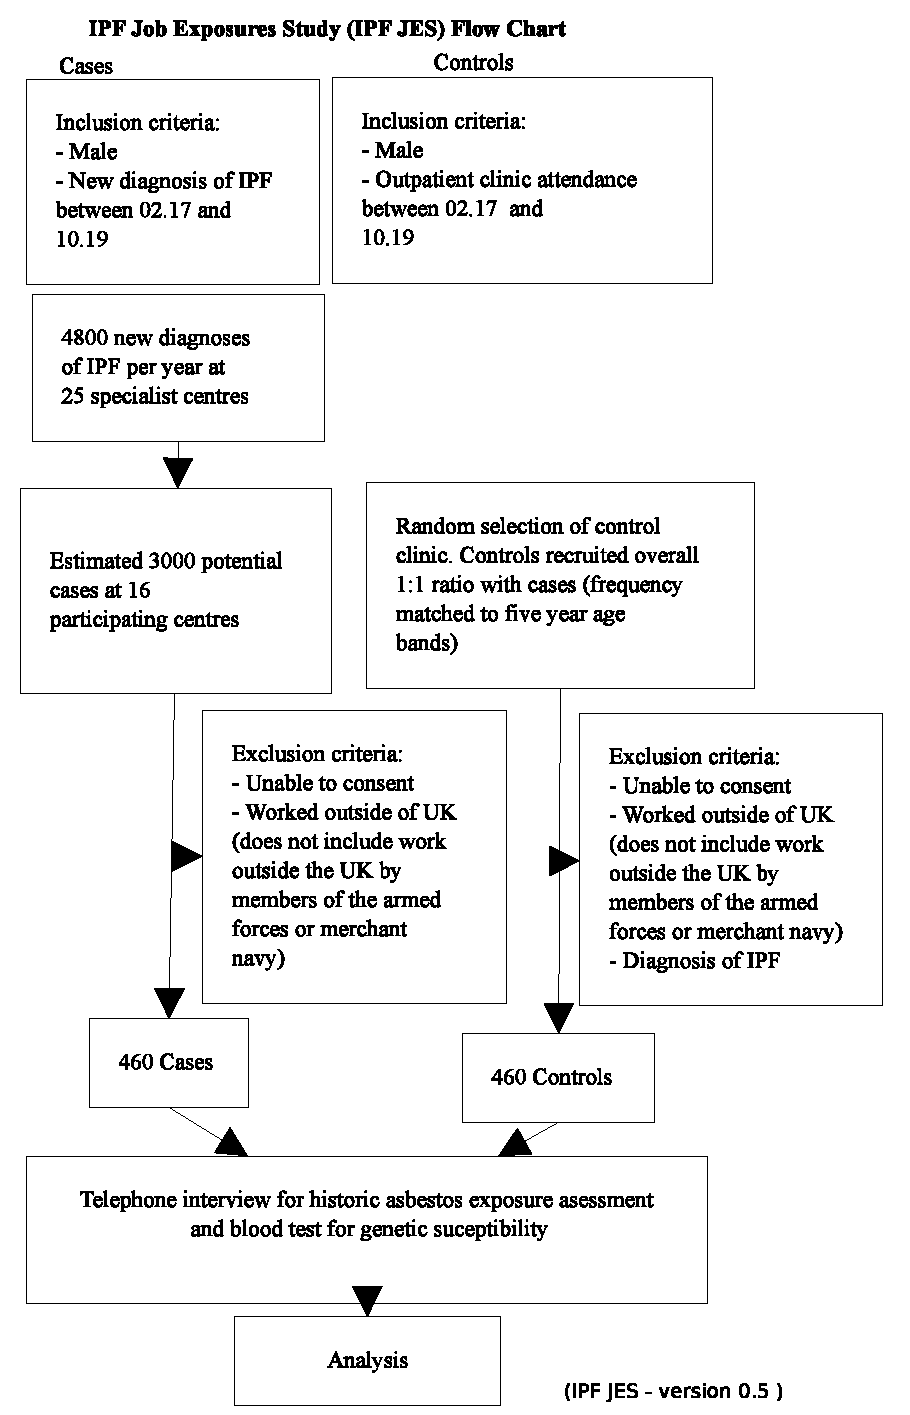
\includepdf[pages={1}]{fig/ipfjes-flowchart.pdf}
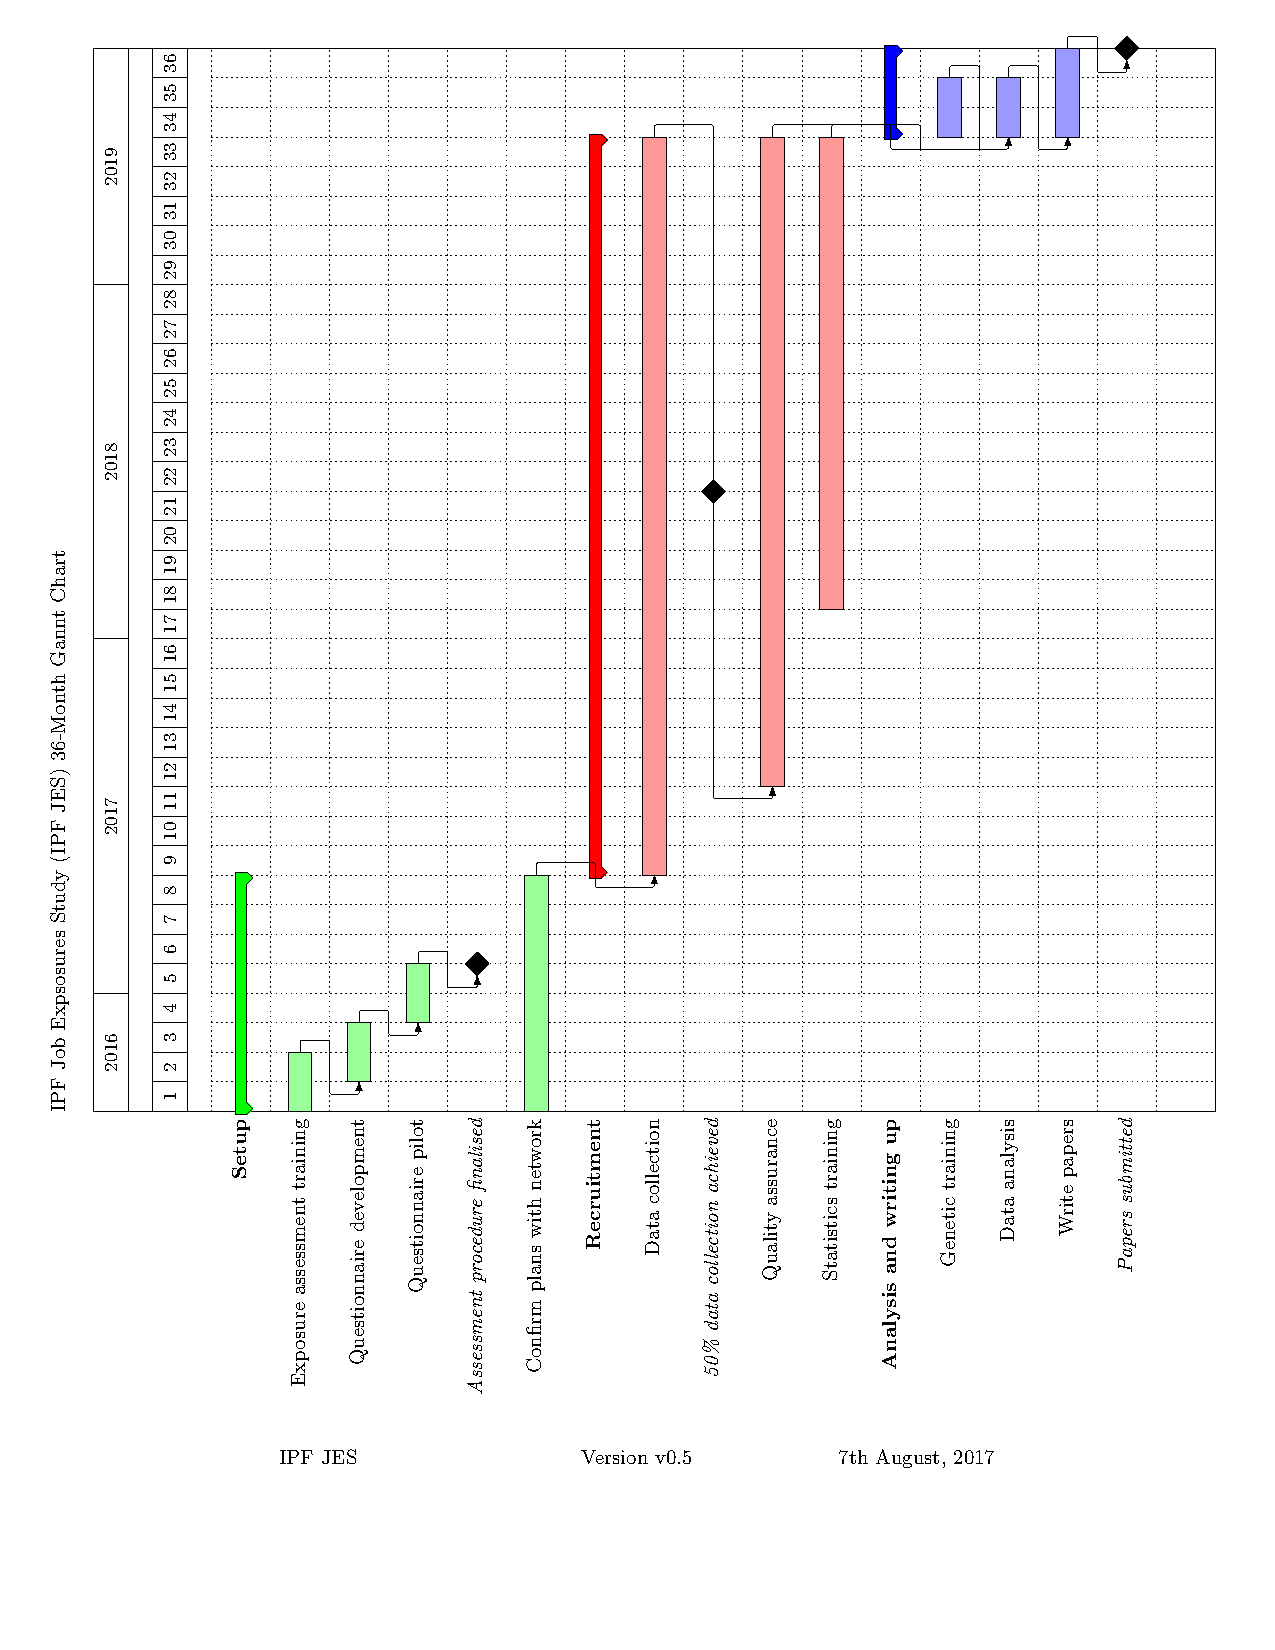
\includepdf[pages={1}]{ipfjes-ganttchart.pdf}

\section{Study Information Sheet for Health Care Professionals}
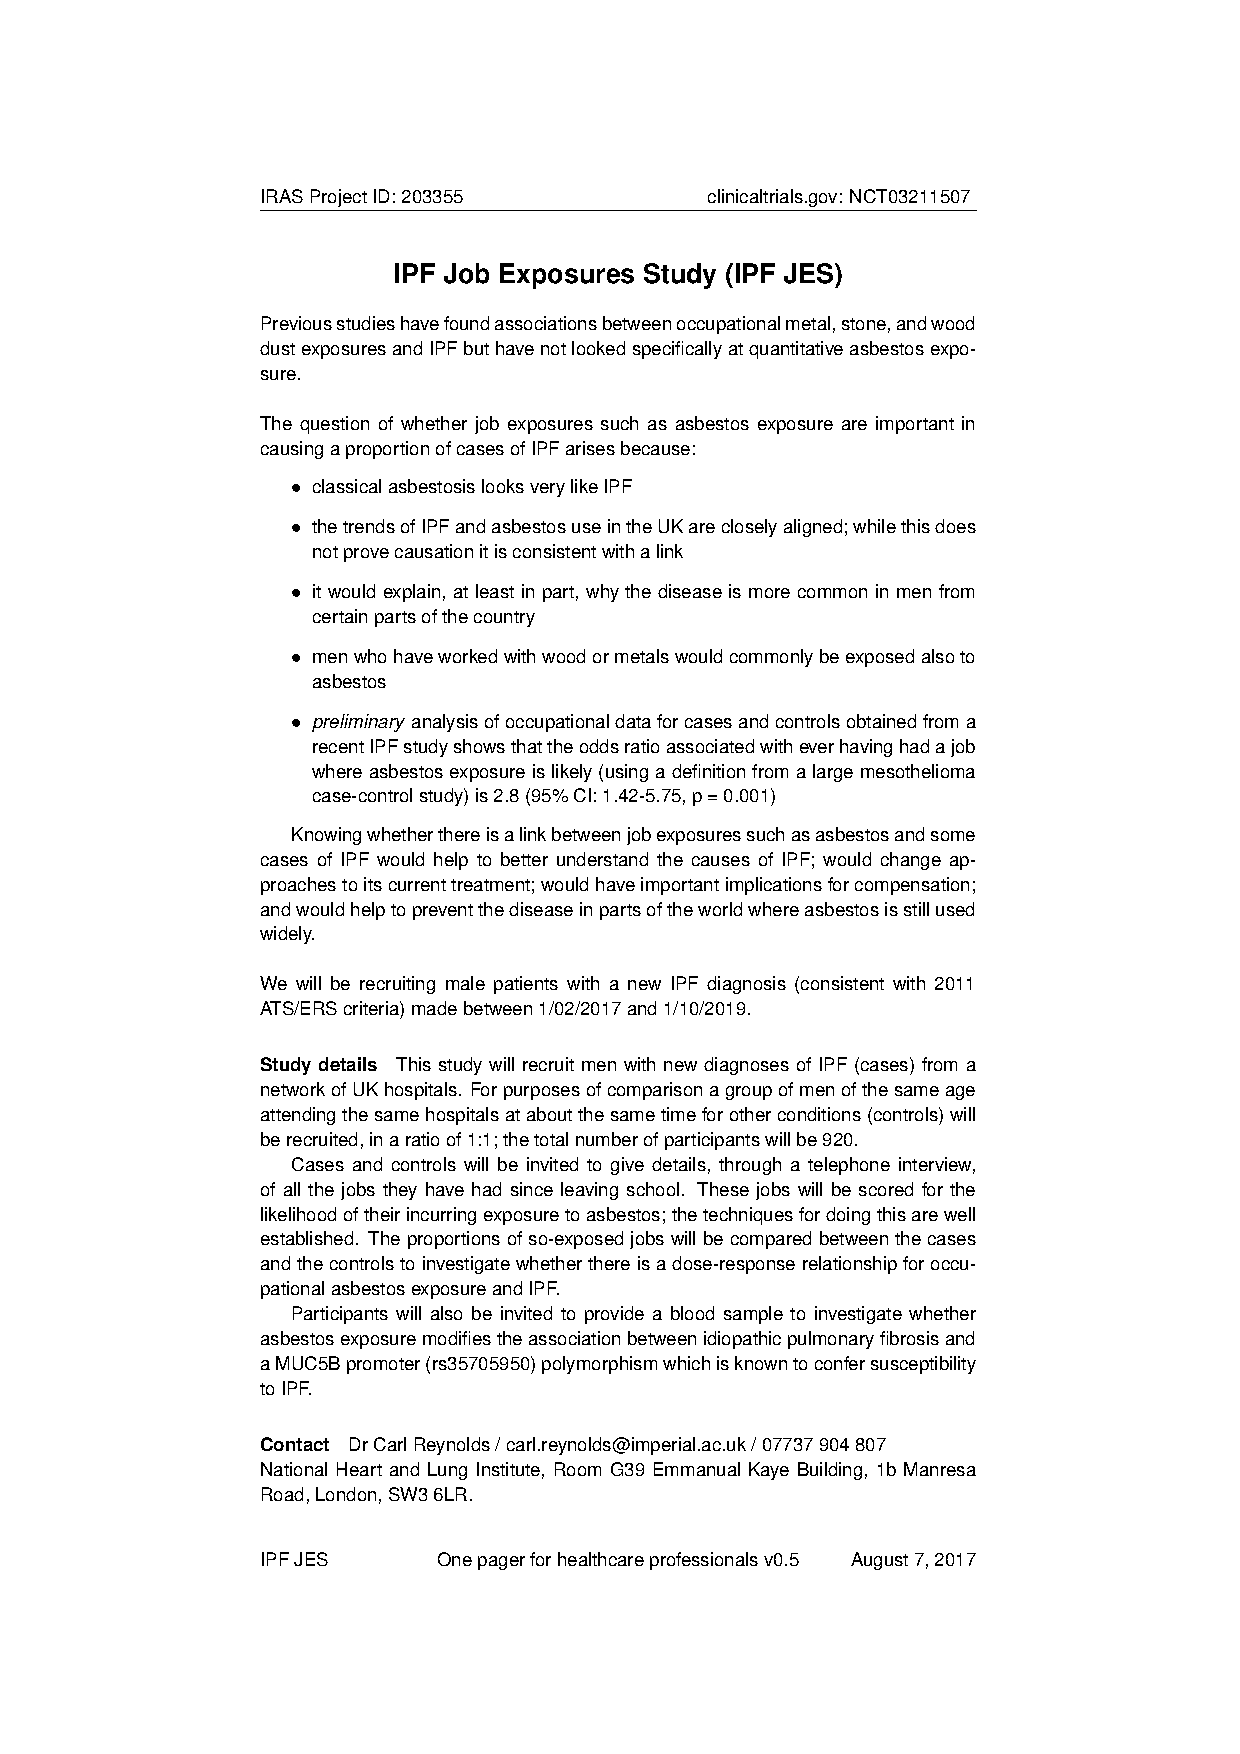
\includepdf[pages={1}]{ipfjes-onepager.pdf}
 \newpage

\section{Participant cover letter template (optional)}
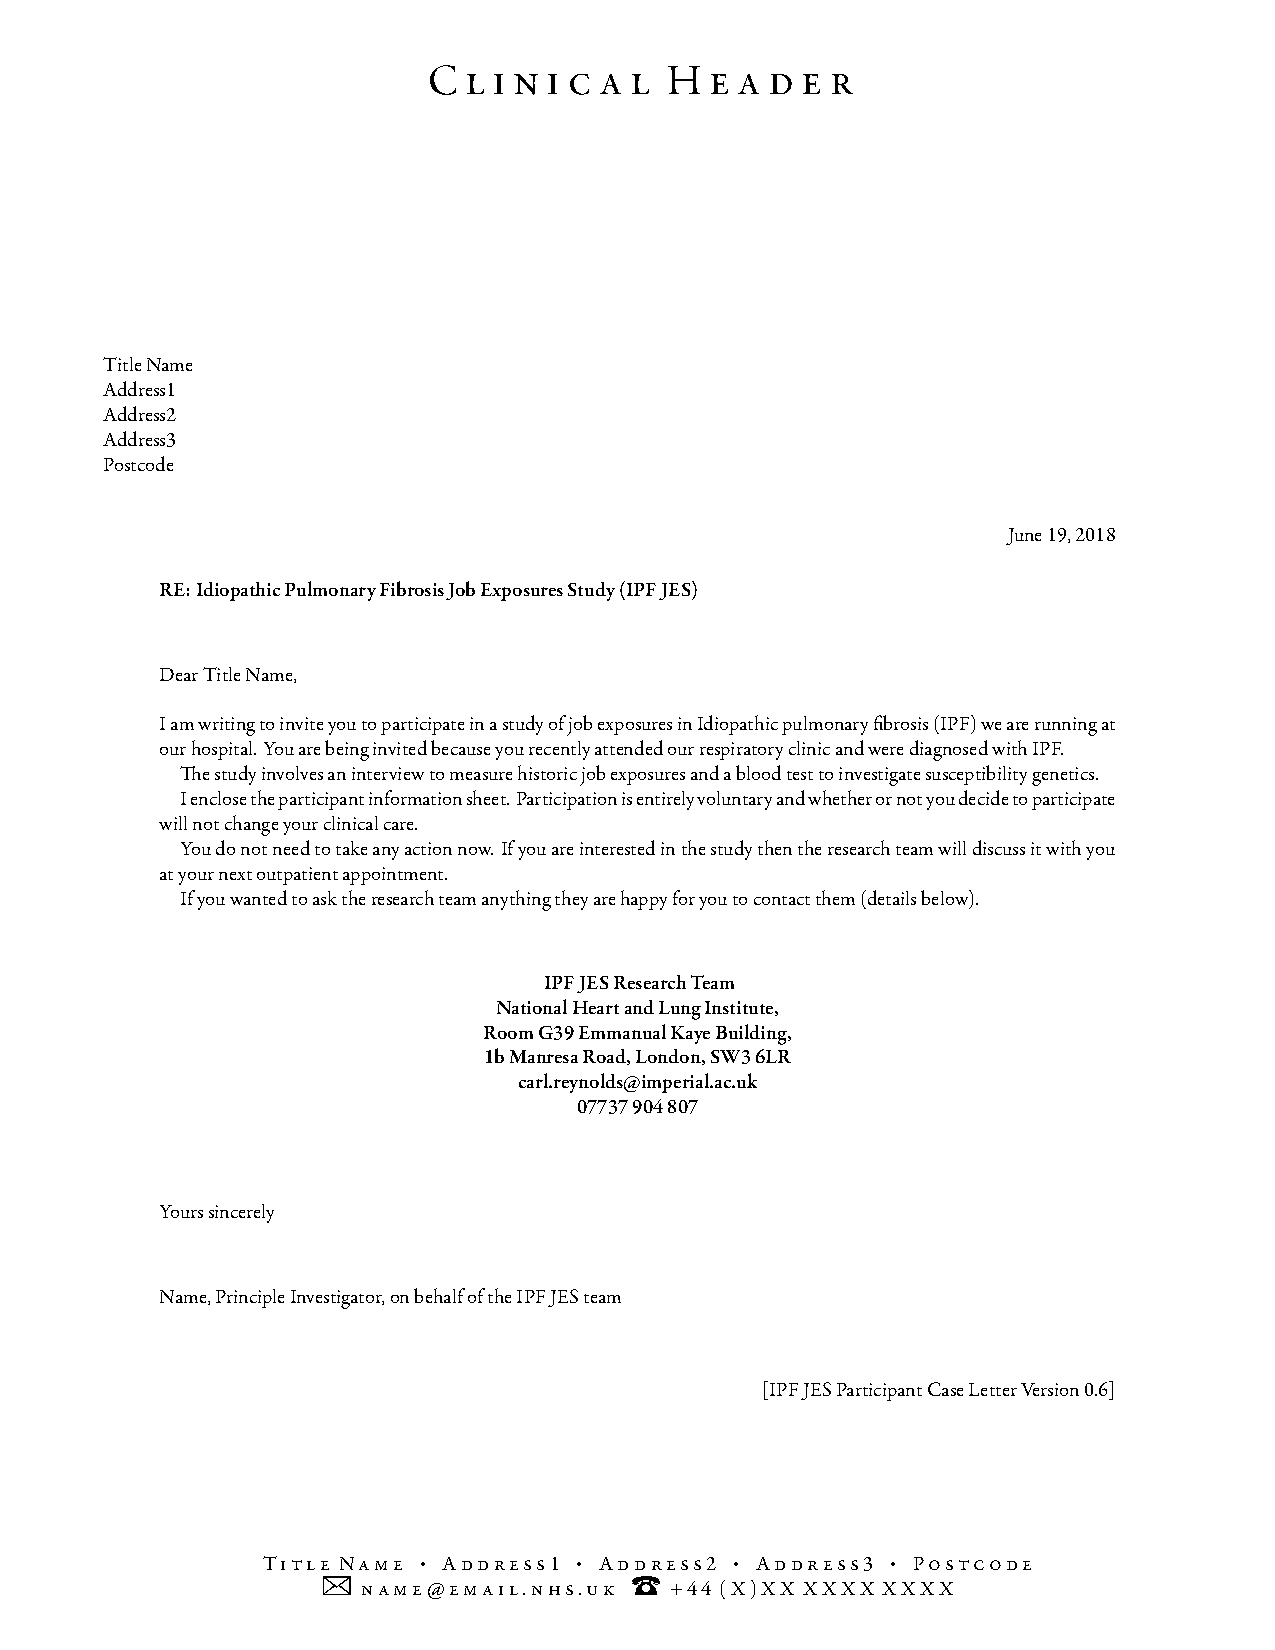
\includepdf[pages={1}]{ipfjes-coverletter-pt.pdf}
\newpage


\section{Participant Information Sheet}
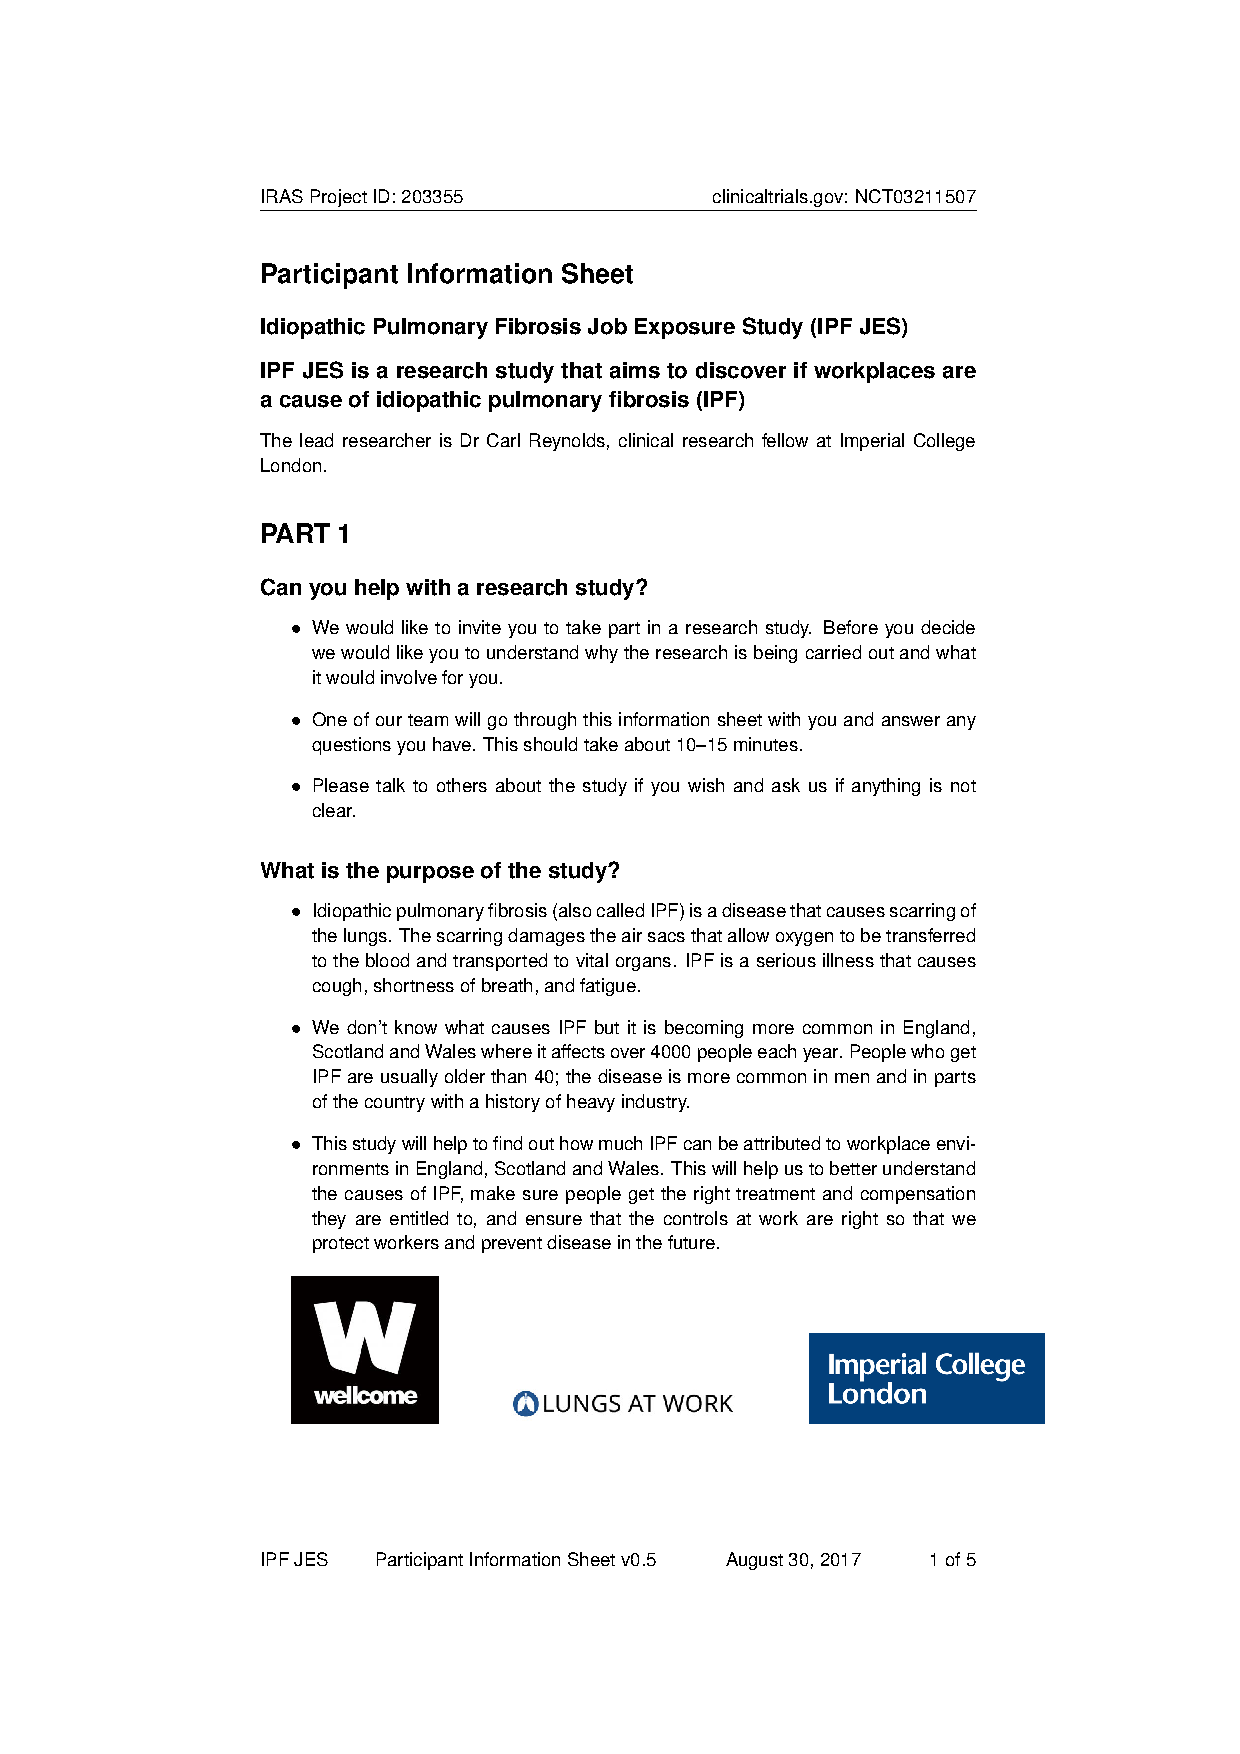
\includepdf[pages={1-5}]{ipfjes-pis.pdf}	
\newpage

\section{Participant consent form}
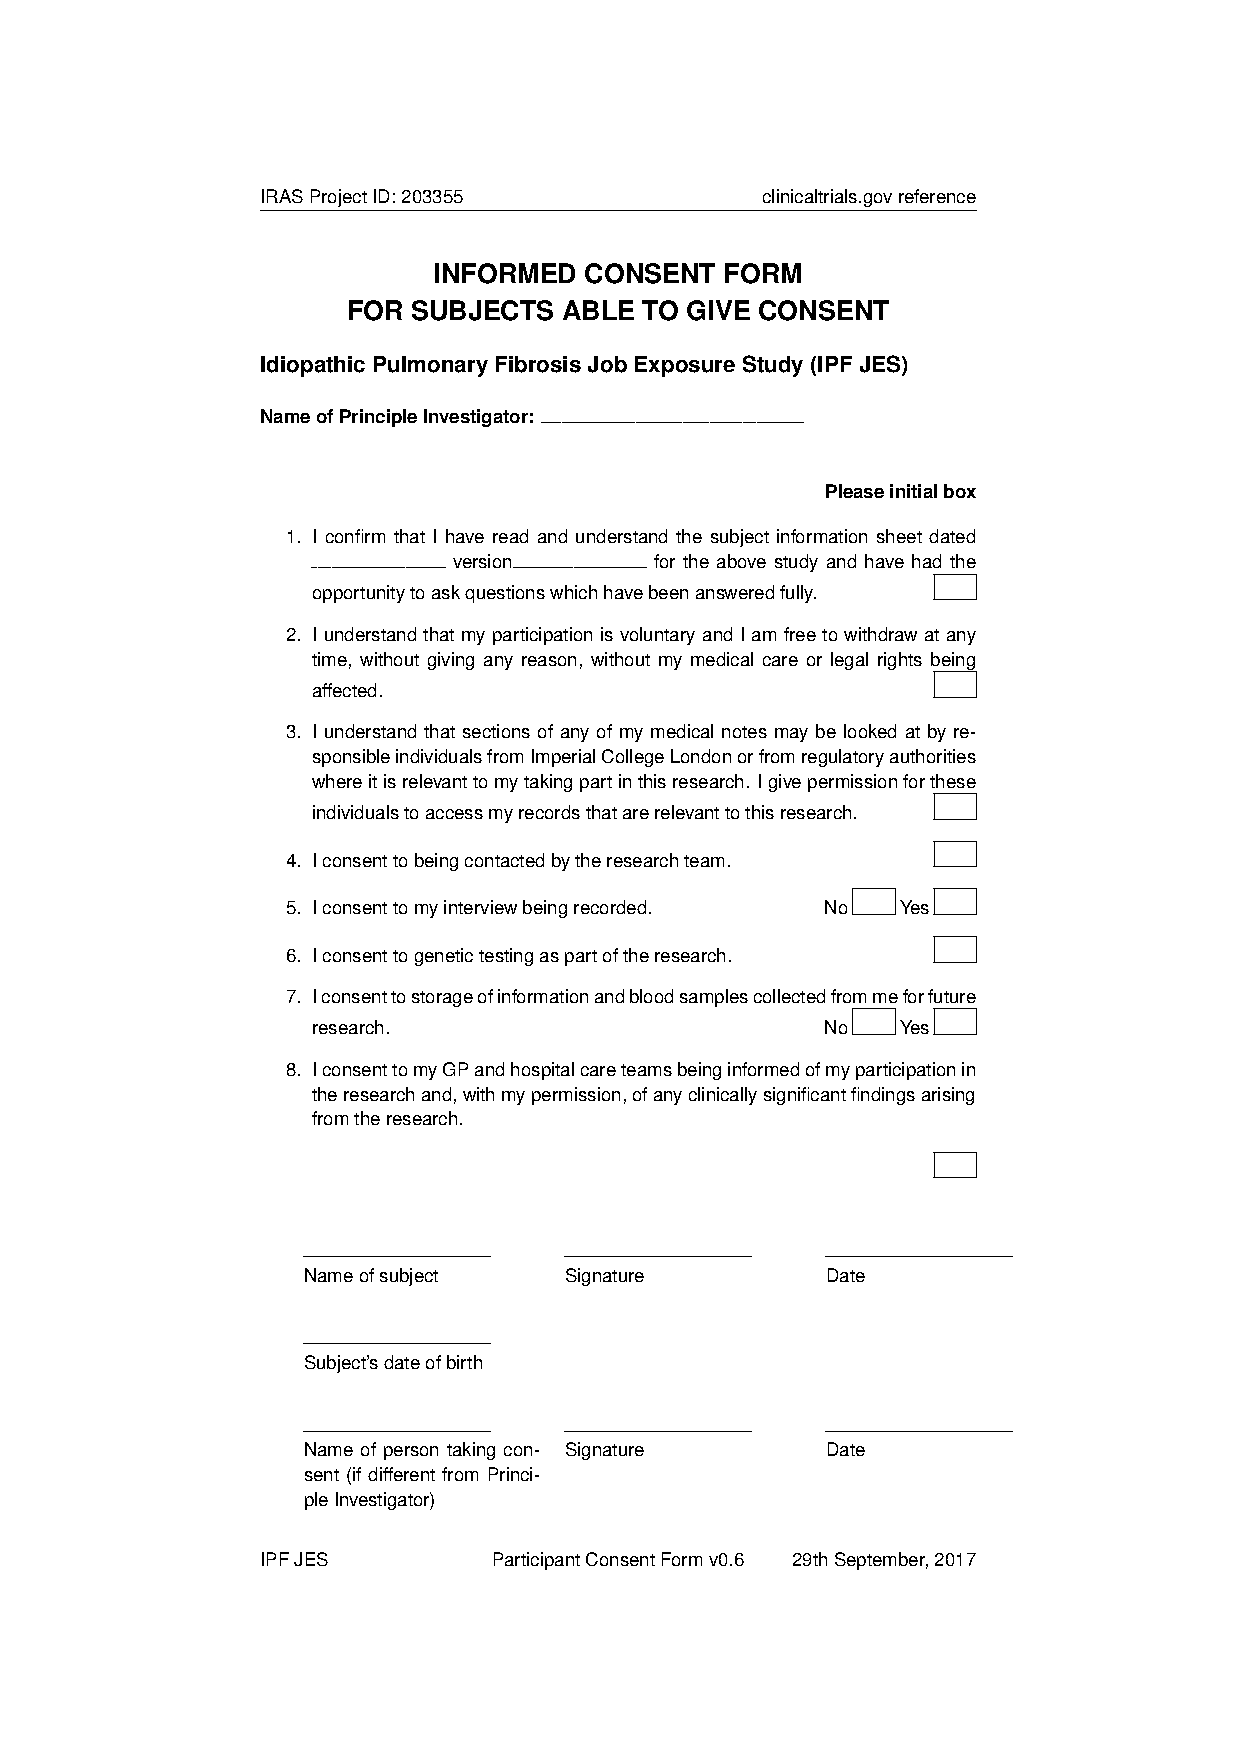
\includepdf[pages={1}]{ipfjes-consent.pdf}
\newpage

\section{Participant job sheet}
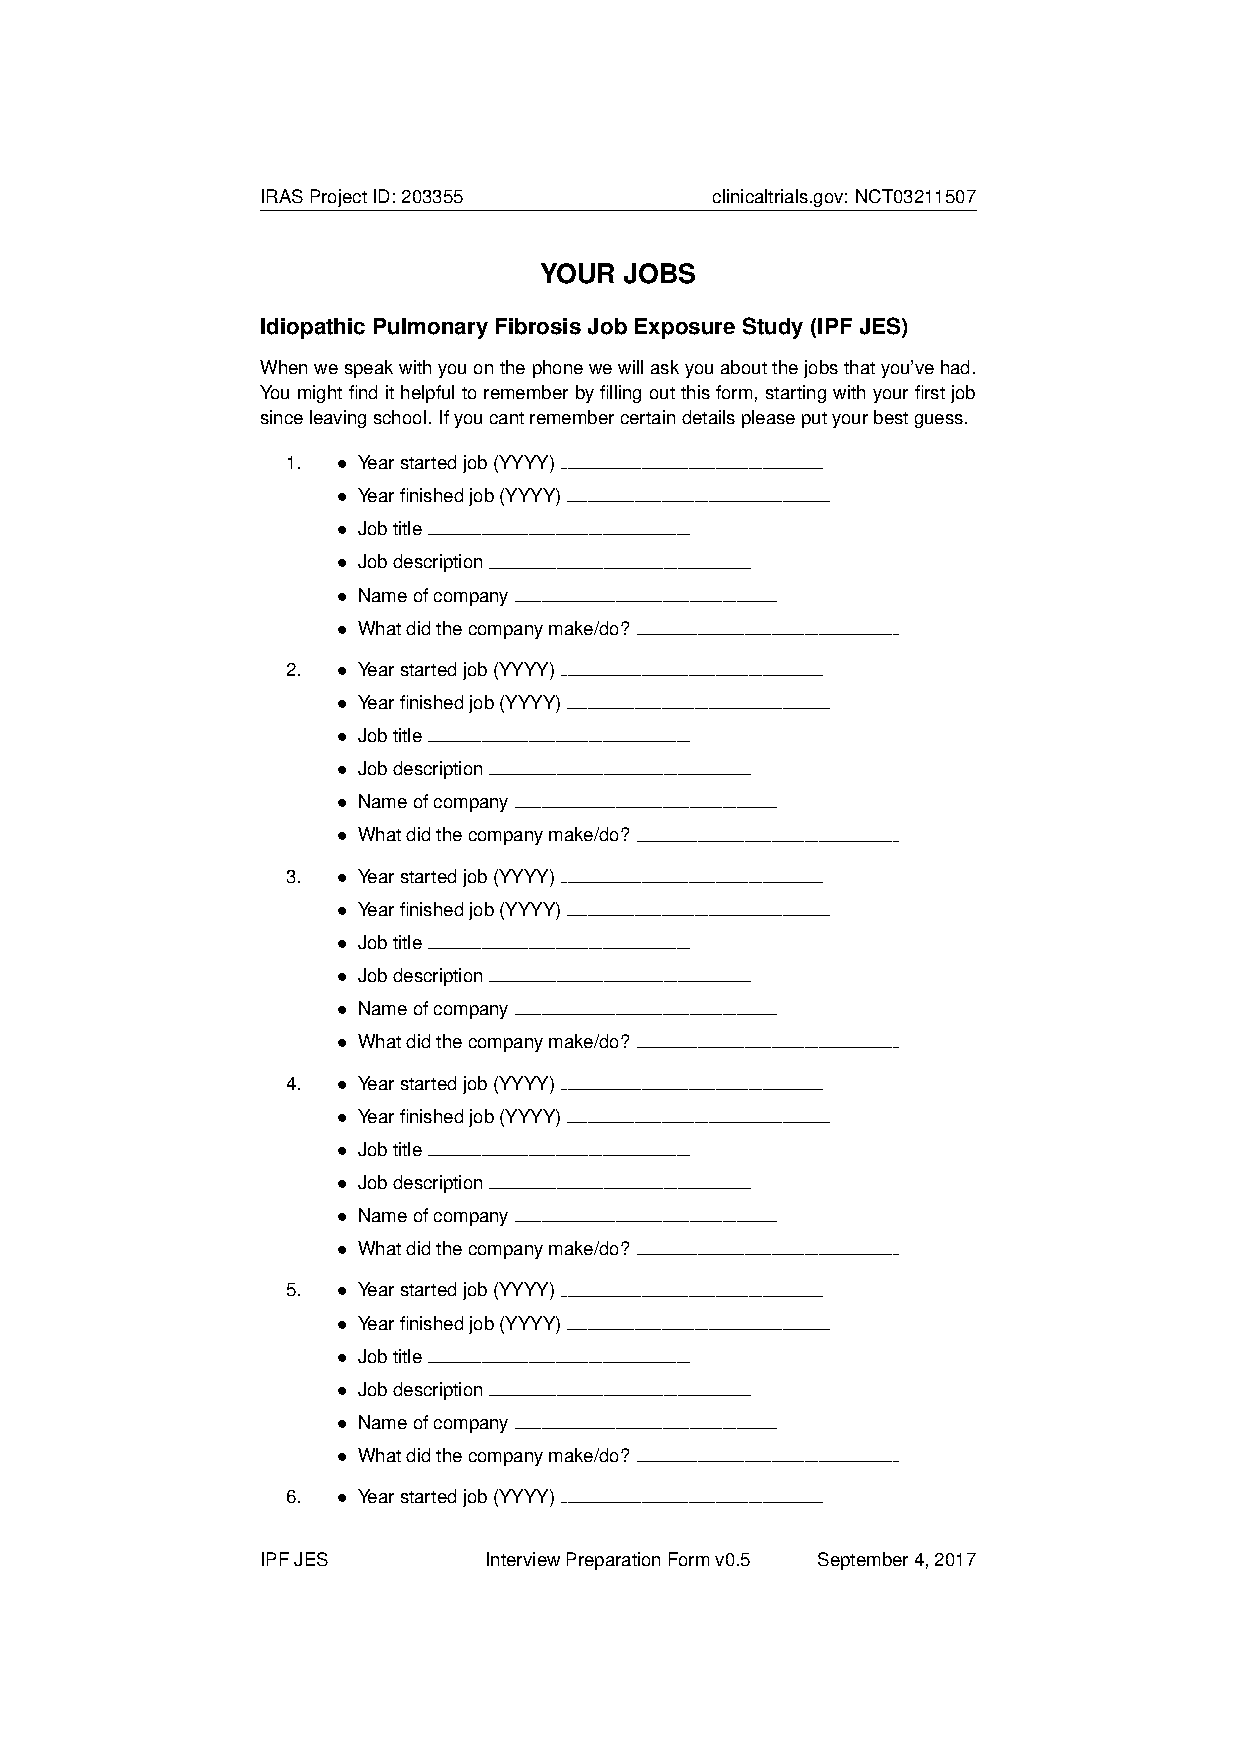
\includepdf[pages={1-4}]{ipfjes-jobs.pdf}
\section{Hospital specialist cover letter (control recruitment)}
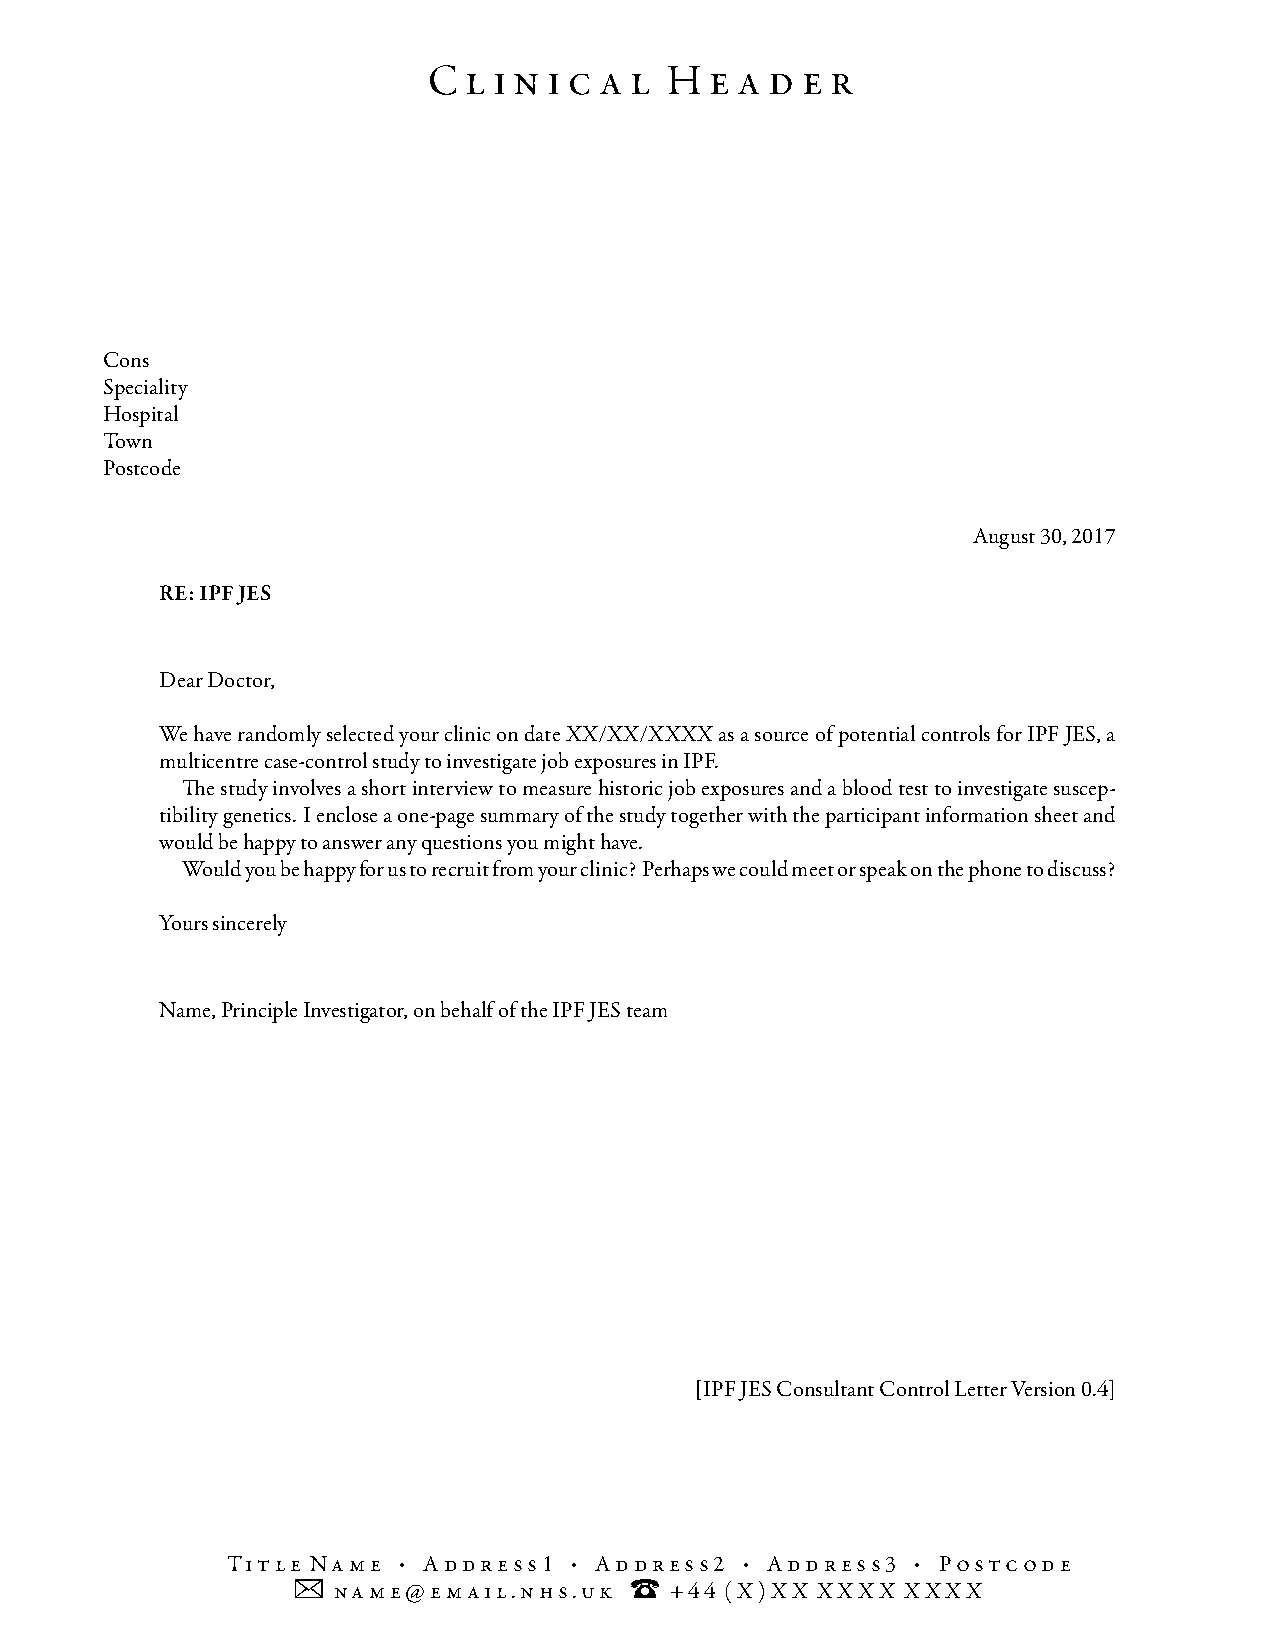
\includepdf[pages={1}]{ipfjes-coverletter-cons-control.pdf}
\newpage

\section{GP cover letter}
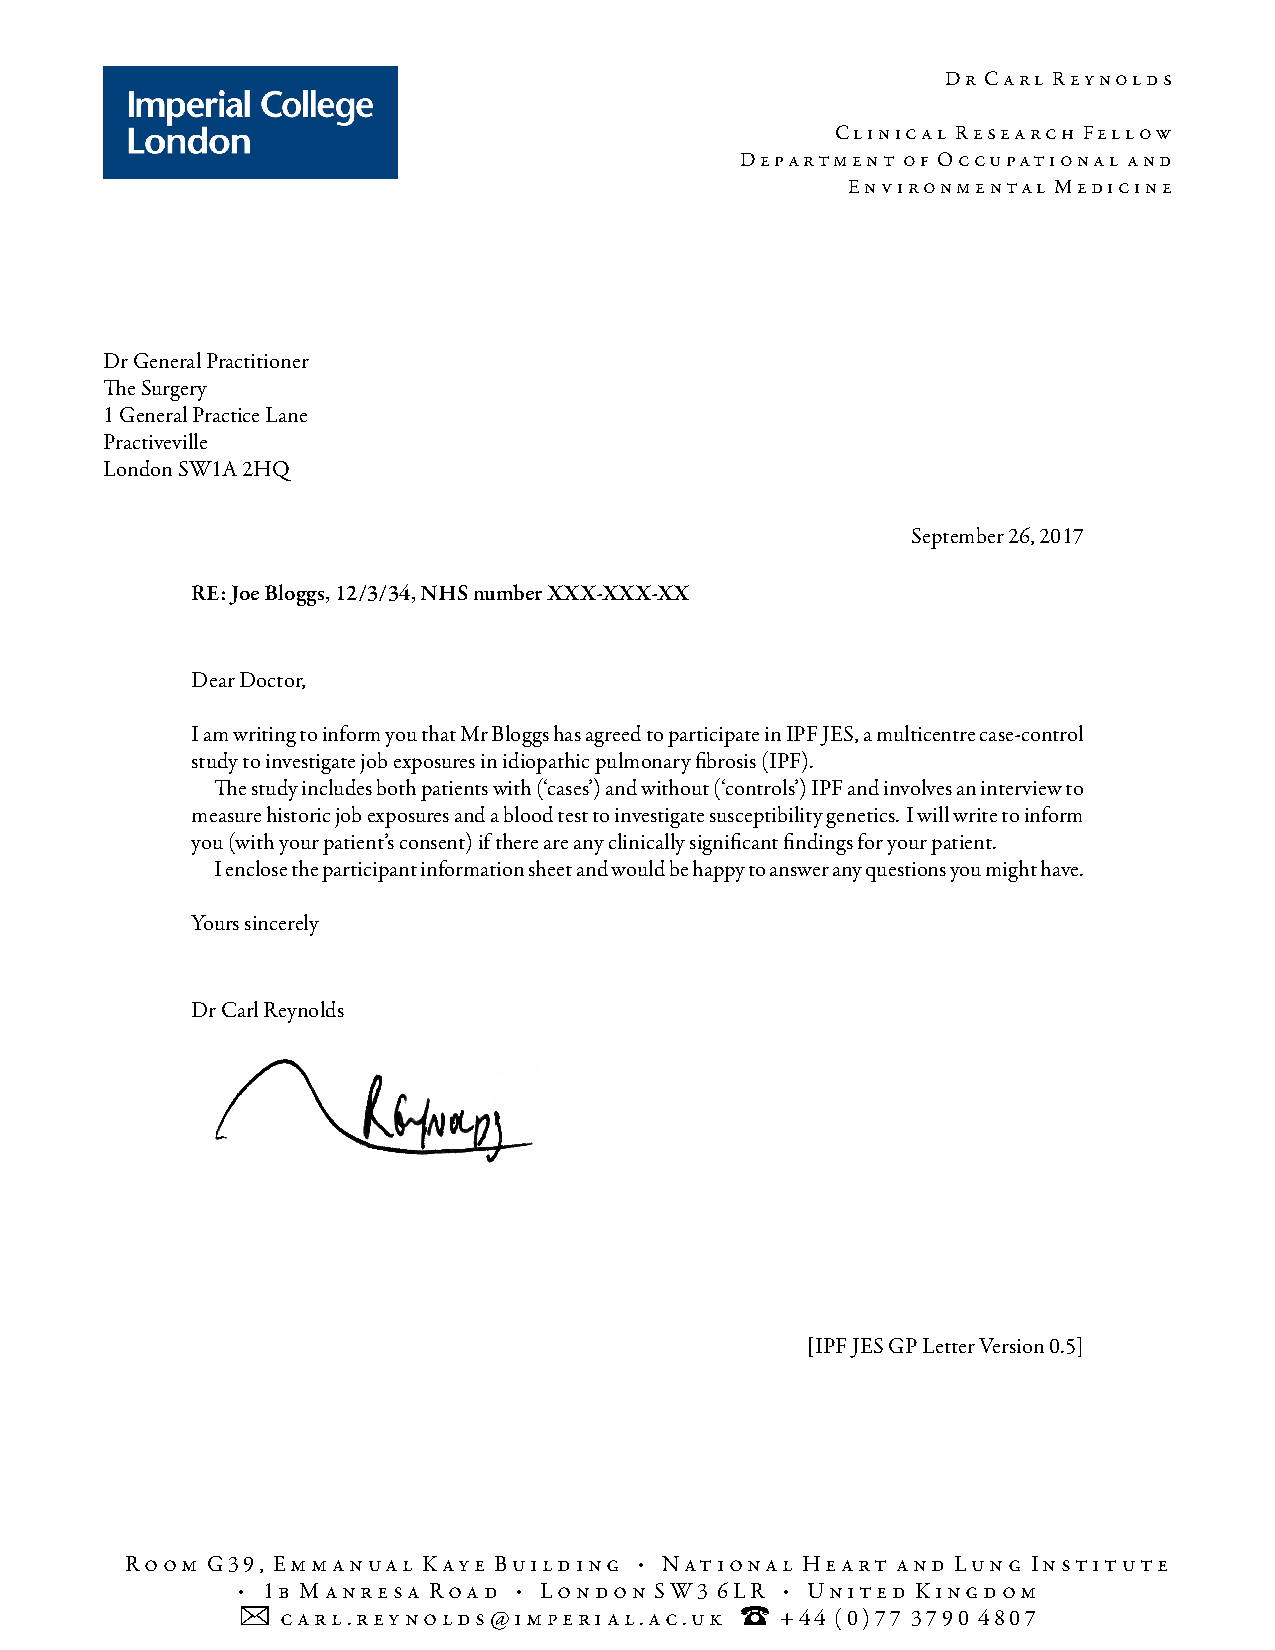
\includepdf[pages={1}]{ipfjes-coverletter-gp.pdf}
\newpage

\section{Study standard operating procedure}
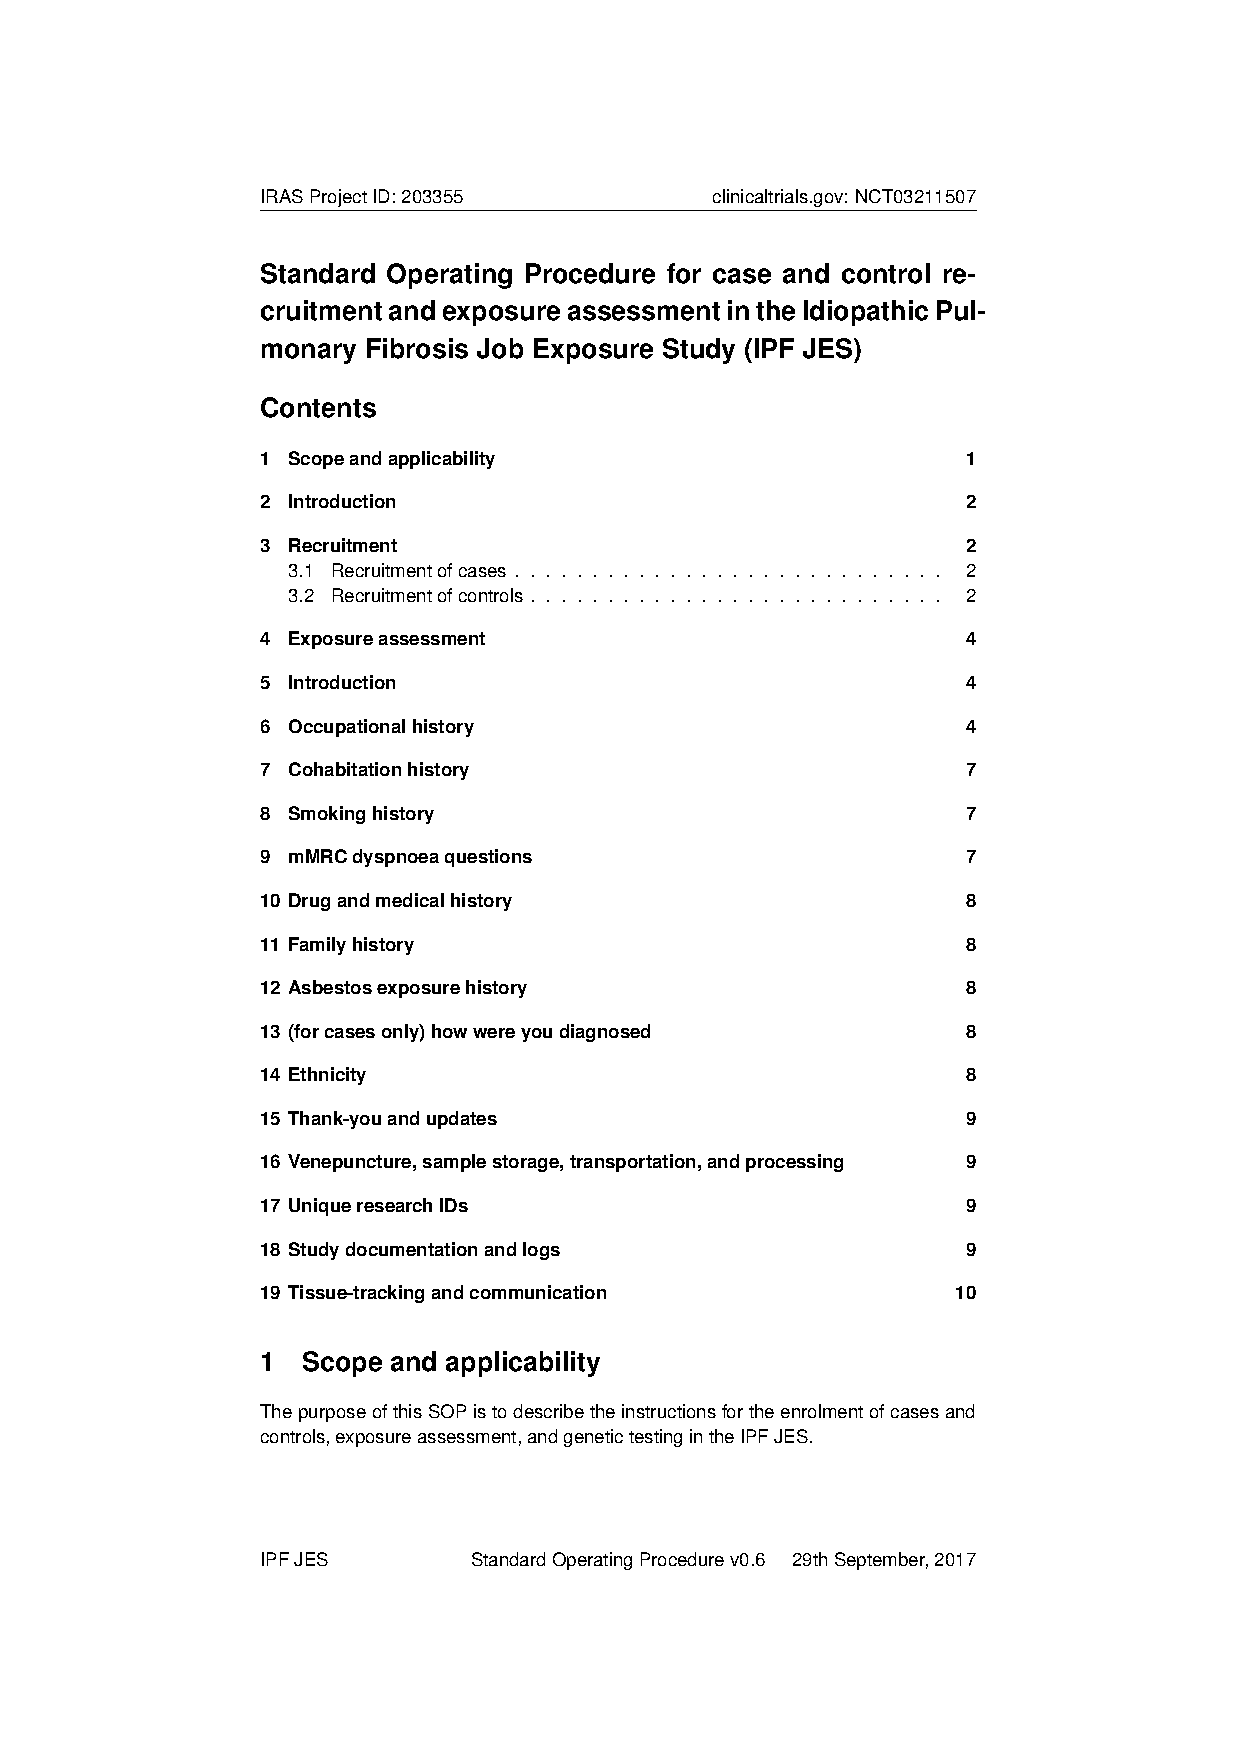
\includepdf[pages={1-6}]{ipfjes-sop.pdf}
\newpage


\end{appendices}
     
%%%%%%%%%%%%%%%%%%%%%%%%%%
\makeatletter
 \def\@biblabel#1{#1}
\makeatother
%%%%%%%% gets rid of bracket around numbers in bibliography
%%%%%%%%%%%%%%%%%%%%%%%%%%%

\bibliographystyle{unsrtnat}
\bibliography{ipfjes}


\end{document}
